\documentclass[11pt]{article}
\usepackage{fullpage}
\usepackage{graphicx}
\usepackage[margin=0.75in]{geometry}



\begin{document}


\begin{center}
    \Large{Intermediate Report }\\
    \large{Angel Dhungana, Avram Twitchell}
    
\end{center}
For the Intermediate report, we ran the Assignment Clustering to cluster the songs based on their loudness and pitches dataset. Then, using the clusters, we took out the top 2 most common artist names and years just to see if there exists a relationship between the artists and the year. For clustering, every row represented a track, and each column represented an audio feature. For this report, we just ran Llyod's Algorithm with K++ and Gonzalez algorithm serving as the the provider for the initial centers. 


\begin{center}
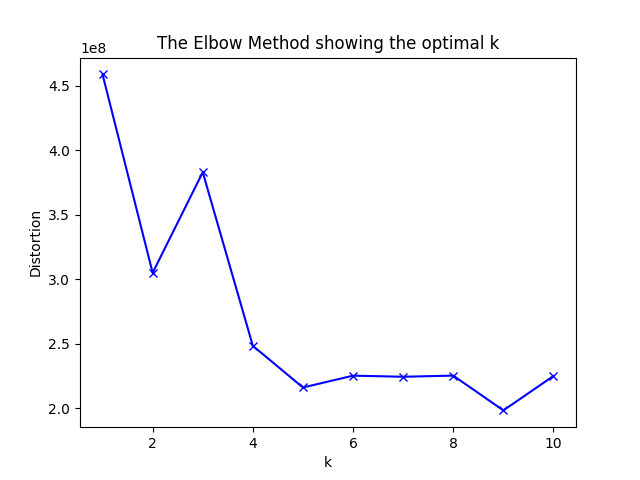
\includegraphics[scale=0.25]{assests/elbowloud.png}
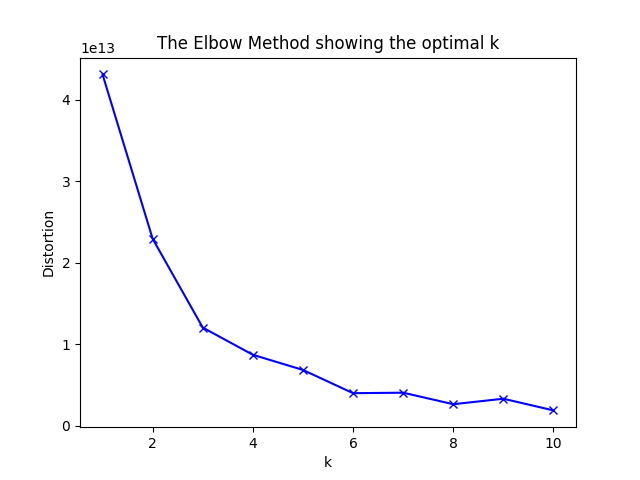
\includegraphics[scale=0.25]{assests/elbowpitches.png}
\end{center}
To get the optimal k for K-Means Clustering, we calculated the sum squared error for each k on the dataset, and plotted it. The k where the plot makes an elbow arc is the optimal k. For loudness dataset, the optimal k was 4 and the for pitches dataset, the optimal k was 3 respectively.


\begin{center}
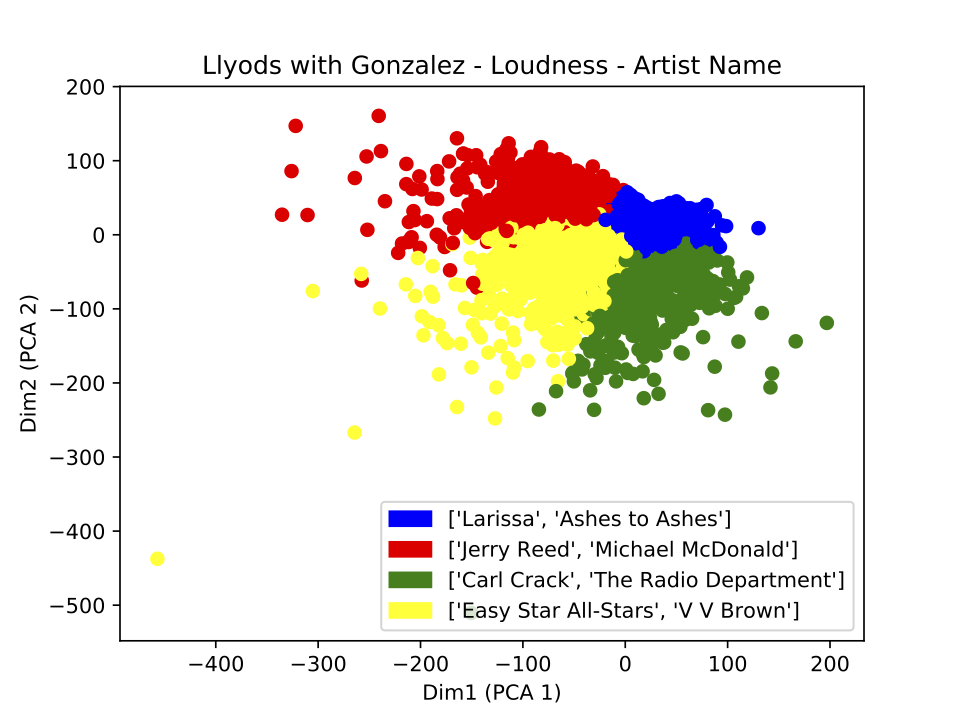
\includegraphics[scale=0.3]{assests/fig1.png}
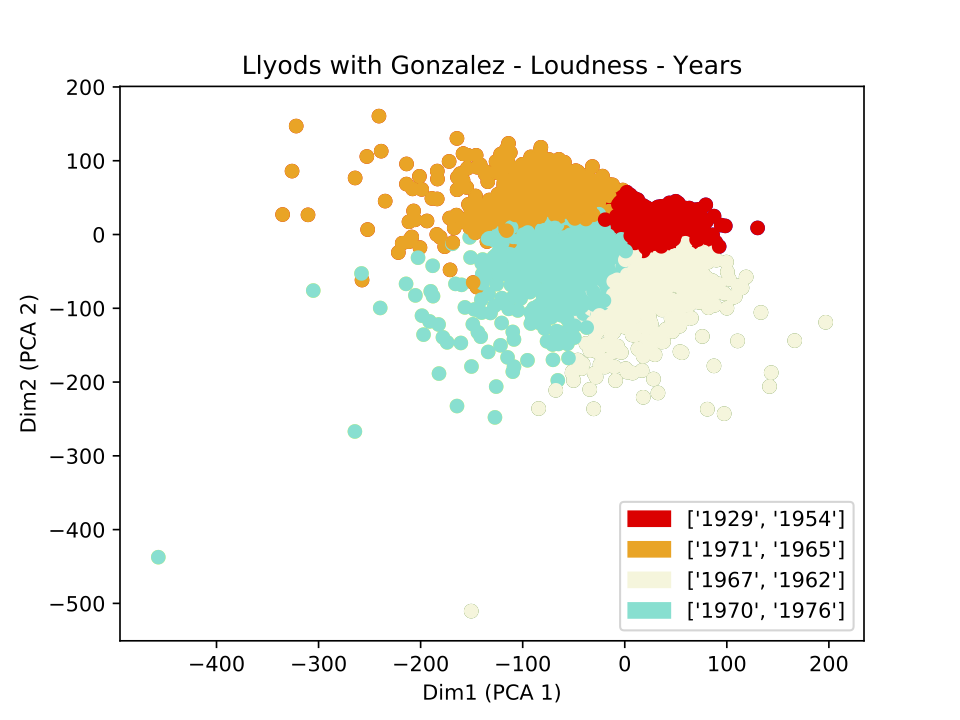
\includegraphics[scale=0.3]{assests/fig2.png}
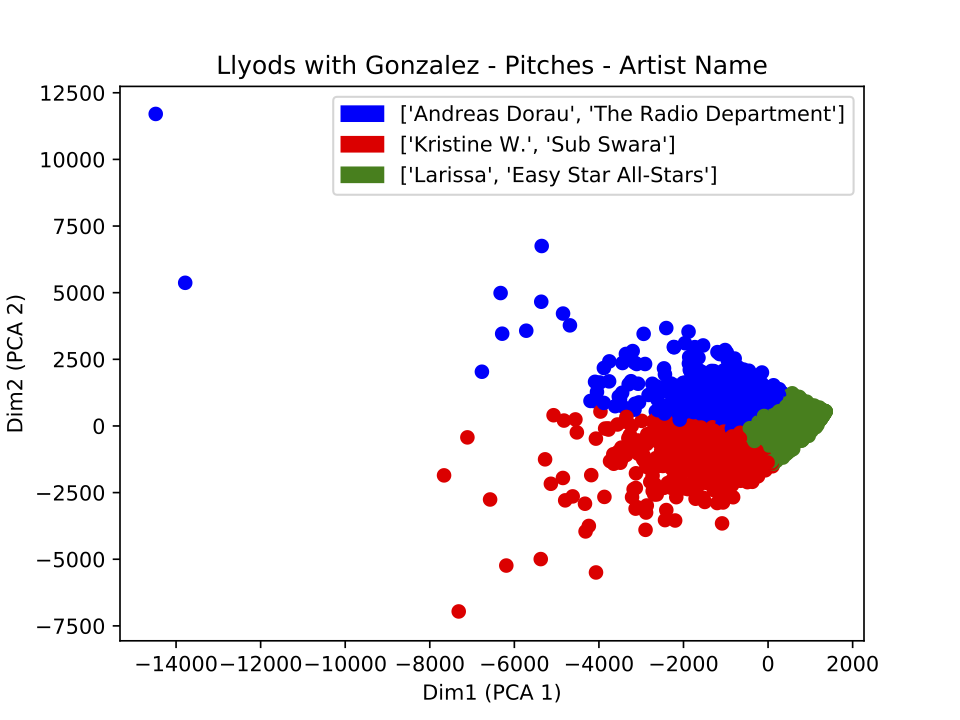
\includegraphics[scale=0.3]{assests/fig3.png}
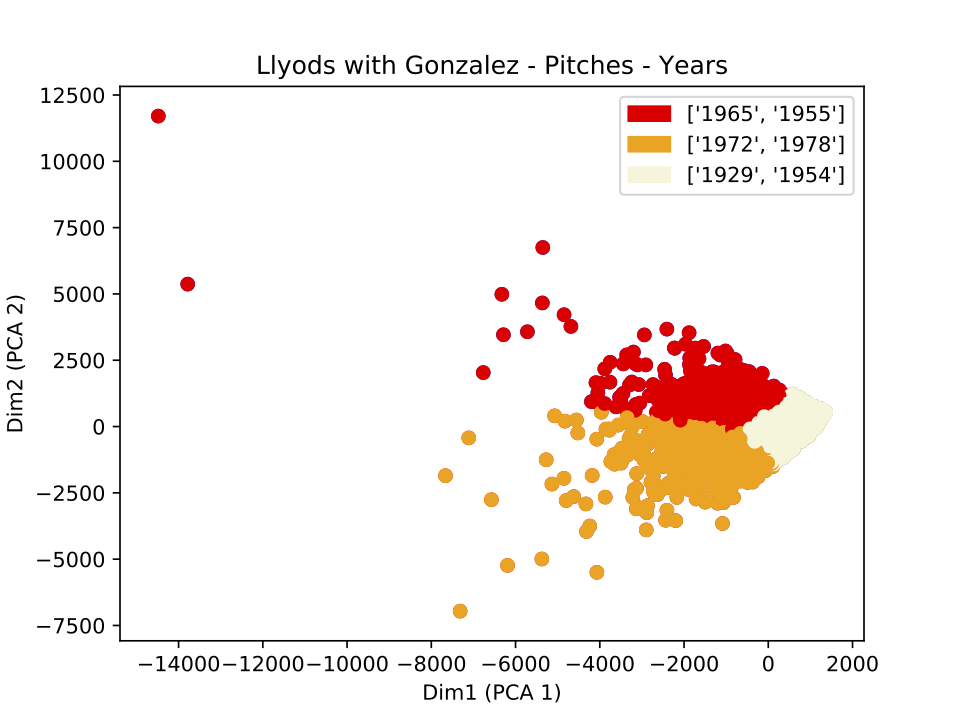
\includegraphics[scale=0.3]{assests/fig4.png}
\end{center}

\begin{center}
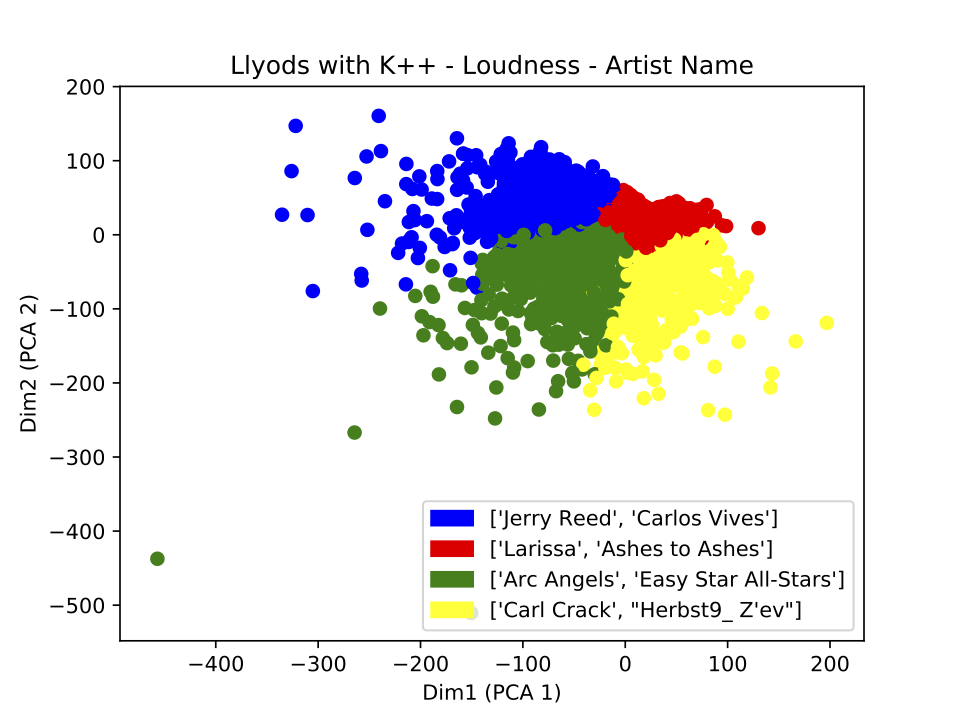
\includegraphics[scale=0.3]{assests/fig5.png}
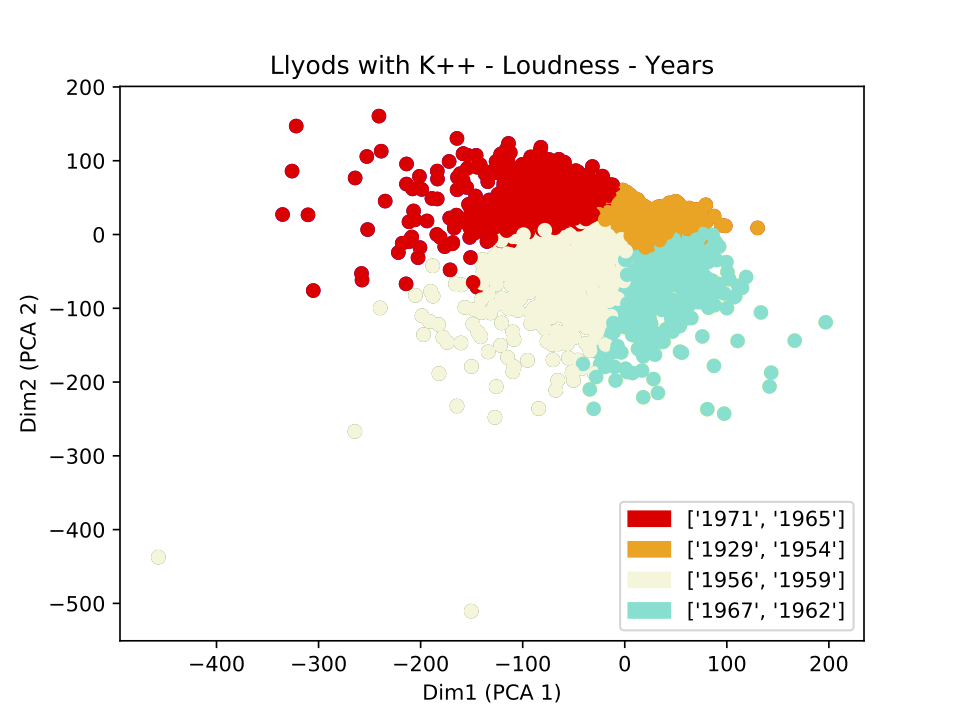
\includegraphics[scale=0.3]{assests/fig6.png}
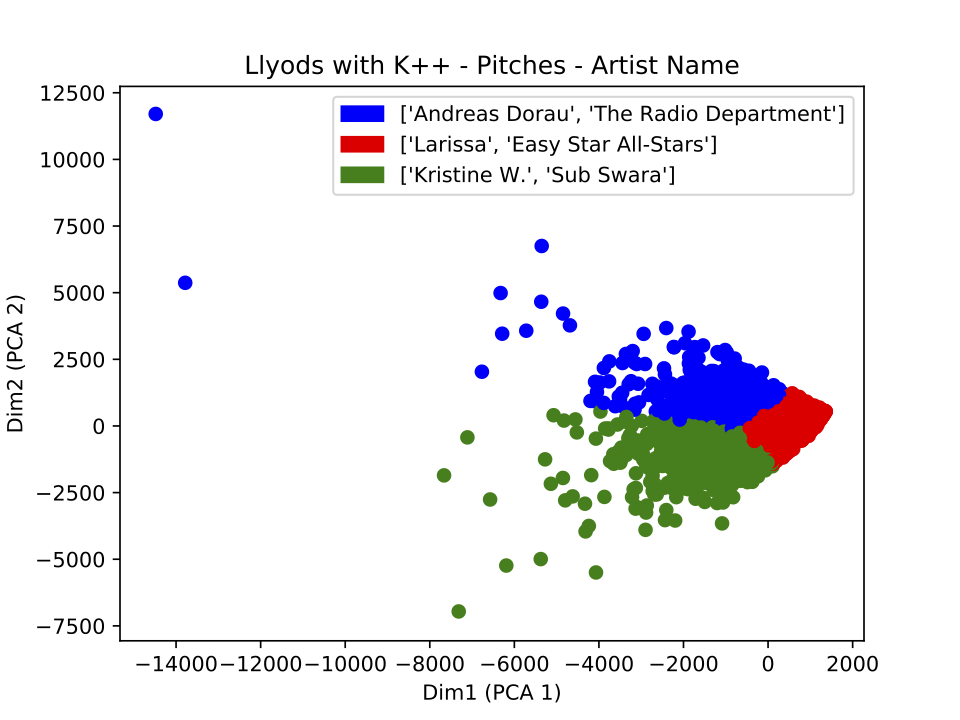
\includegraphics[scale=0.3]{assests/fig7.png}
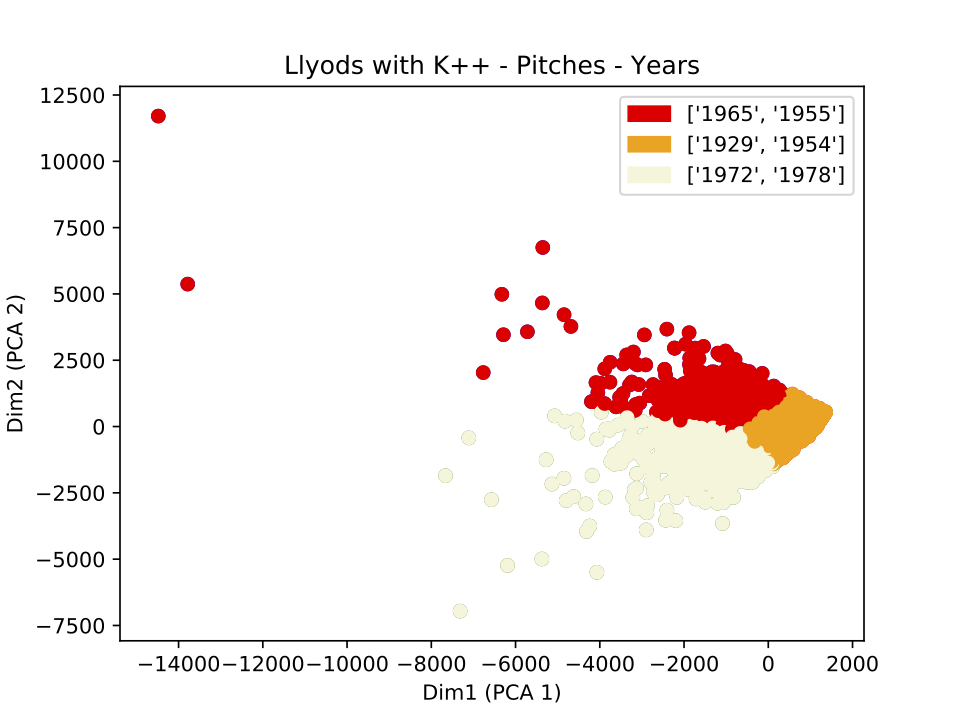
\includegraphics[scale=0.3]{assests/fig8.png}
\end{center}

The loudness and pitches dataset had a large range of columns. Hence, for the visualization purpose we used the PCA to reduce the dataset dimension to 2, and plotted the graph based on it. From the graph, we can see that the Gonzalez and K++ don't have any significant differences but we can see some of the outlier tracks are being classified into different clusters. Thus, \textit{K++ will work well overall in general.}

\begin{itemize}
\item Pitches vs Loudness
\begin{itemize}
	\item Only one artist name came up as the most common in both dataset clusters. And its 'Larissa'. Based on the Loudness cluster, "Larissa' is most similar to 'Ashes to Ashes' and based on Pitches cluster, 'Larissa' is most similar to 'Easy Star All-Stars'. 
	\item We can see that '1929' and '1954' appear both on Loudness as well as Pitches graph as the top 2 most common. Hence, we can conclude that the songs of the year 1929 and 1954 were the most similar based both on their loudness and pitches.
	\item We can also see that based on the pitches, the year '1965' was most similar to '1955' while with loudness, the year '1971' was most similar to '1965'. 
\end{itemize}
\item This experiment was done by separating loudness and pitches into different graphs, however for the final report, we might want to do Loudness vs Pitches with each representing X and Y axis respectively, to demonstrate the effectiveness in full dataset.
\end{itemize}


\end{document}
